\documentclass[a4paper]{article}
\usepackage[14pt]{extsizes} 
\usepackage[T2A]{fontenc}
\usepackage[utf8]{inputenc}
\usepackage{natbib}
\usepackage{graphicx}
\usepackage{amsmath}
\usepackage[english]{babel}
\usepackage{fontspec}
\usepackage{amsmath,amsfonts,amssymb,amsthm,mathtools,mathrsfs}
\usepackage{icomma}
\usepackage{fullpage}
\usepackage{ulem}
\usepackage{eufrak}
\usepackage{setspace}
\usepackage{listings}
\usepackage{indentfirst}
\usepackage[left=2cm,right=1.5cm,top=2cm,bottom=2cm]{geometry}
\usepackage{xcolor}
\usepackage{float}
\usepackage{csquotes}

\setmainfont[Ligatures={TeX,Historic}]{Times New Roman}
\setlength{\parindent}{5ex}
\setlength{\parskip}{1em}
\renewcommand{\baselinestretch}{1}

\graphicspath{{images/}}

\definecolor{buzzlightyear}{HTML}{8757A5}
\definecolor{grass}{HTML}{738D06}
\definecolor{literal}{HTML}{F18A2B}
\definecolor{commentcolor}{HTML}{8E908B}

\lstdefinestyle{habrstyle}{
    backgroundcolor=\color{white},   
    commentstyle=\color{commentcolor},
    keywordstyle=\bfseries\color{buzzlightyear},
    numberstyle=\tiny\color{commentcolor},
    stringstyle=\color{grass},
    basicstyle=\ttfamily\footnotesize,
    breakatwhitespace=false,         
    breaklines=true,                 
    captionpos=b,                    
    keepspaces=true,                 
    numbers=left,                    
    numbersep=5pt,                  
    showspaces=false,                
    showstringspaces=false,
    showtabs=false,                  
    tabsize=4
}

\lstset{style=habrstyle}

\begin{document}

    % FIRST PAGE
    \begin{center}
        \begin{center}
        \hfill \break
        \normalsize{Санкт-Петербургский государственный политехнический}\\
        \normalsize{университет Петра Великого}\\
        \hfill \break
        \normalsize{\textbf{Высшая школа интеллектуальных систем и}}\\ 
        \normalsize{\textbf{суперкомпьютерных технологий}}\\ 
        \hfill \break
        \hfill \break
        \hfill \break
        \normalsize{Лабораторная работа}\\
        \hfill \break
        \hfill \break
        \normalsize{\LARGE Дискретное преобразование Фурье}\\
        \end{center}
        \hfill \break
        \hfill \break
        \hfill \break
        \hfill \break
        \hfill \break
        \hfill \break
        \hfill \break
        \hfill \break
        \hfill \break
        \hfill \break
        \begin{flushright}
            \normalsize{Работу выполнил студент}\\
            \normalsize{3-го курса, группа 3530901/80201}\\
            \normalsize{Сахибгареев Рамис Ринатович}\\
            \hfill \break
            \normalsize{Преподаватель:}\\
            \normalsize{Богач Наталья Владимировна}\\
        \end{flushright}
        \hfill \break
        \hfill \break
        \hfill \break
        \hfill \break
        \begin{center} Санкт-Петербург 2021 \end{center}
        \thispagestyle{empty}
    \end{center}
    % FIRST PAGE [END]
    
    \newpage
        \tableofcontents
    
    \newpage
         \listoffigures
    
    \newpage
         \lstlistoflistings   
     
    % START START START START START
    \newpage
        \section{Part 1: Research and execution of chap07}
        
        In this part we need to research and execute existing chap07.ipynb file, that contains information about Complex Signals, DFT and real and imaginary transformations.
        
        File was successfully executed. Complex signal - is a signal, that have real and imaginary parts. They have same frequencies and amplitudes, but different phase (cos and sin signals), so human cannot recognize any difference between them. Also we can rotate the signal, but because different frequencies has different cycle time, signal changes too.
        
        \begin{figure}[H]
            \centering
            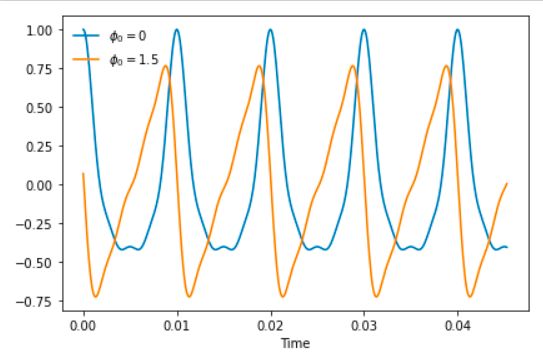
\includegraphics[width=\textwidth]{img/p1_2.png}
            \caption{Phase changing result. Signals are different}
            \label{fig:p1_2}
        \end{figure}
        
        We can also see, that full DFT also has negative frequencies.
        
        \begin{figure}[H]
            \centering
            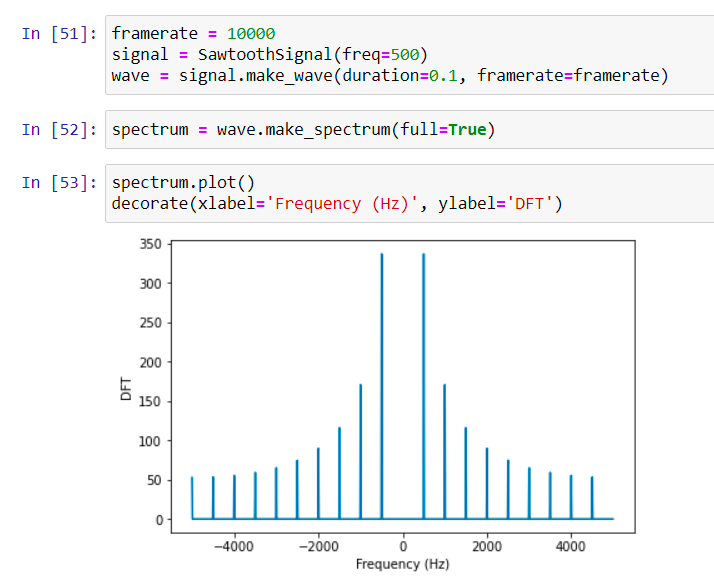
\includegraphics[width=\textwidth]{img/p1_1.png}
            \caption{Full DFT result on a sawtooth signal signal}
            \label{fig:p1_1}
        \end{figure}
        
    \newpage
        \section{Part 2: Fast Fourier Transform (FFT) implementation}

        In this part we need to implement FFT using Damielson-Lancouz lemma. (o) and (e) is arrays, containing odd and even elements of ys correspondingly.
        
        \[ DFT(y)[n] = DFT(e)[n] + exp(-2*\pi*i*n/N) * DFT(o)[n] \]
        
        Standard DFT function take \[N^2\] time to be computed, which is good for a small N, but can take enormous time for big N. That's why we need to use recursive FFT, which takes around \[N*logN\] steps to be computed. When size of iteration will be small, we can use standard DFT, to get needed values.
        
        To implement FFT let's use code of DFT, given in the previous part.
        
        \begin{lstlisting}[language=Python,caption=DFT definition,label={lst:part1_2}]
    def synthesis_matrix(N):
        ts = np.arange(N) / N
        freqs = np.arange(N)
        args = np.outer(ts, freqs)
        M = np.exp(1j * PI2 * args)
        return M
    def dft(ys):
        N = len(ys)
        M = synthesis_matrix(N)
        amps = M.conj().transpose().dot(ys)
        return amps
        \end{lstlisting}
        
        Using it and Damielson-Lancouz lemma let's implement Fast Fourier Transform function.
    
        \begin{lstlisting}[language=Python,caption=FFT definition,label={lst:part1_2}]
    def fft(ys):
        N = len(ys)
        for (i)
        if N <= 4:
            return dft(ys)
        
        even = fft(ys[::2])
        odd = fft(ys[1::2])
                
        ns = np.arange(N)
                
        return np.tile(even, 2) + np.exp(-1j * PI2 * ns / N) * np.tile(odd, 2)
        \end{lstlisting}
        
        And we can compare its result to np.fft.ftt.
        
        \begin{figure}[H]
            \centering
            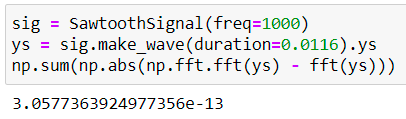
\includegraphics[width=\textwidth]{img/p2_1.png}
            \caption{FFT testing}
            \label{fig:part1_1_2}
        \end{figure}
        
        We can see, that difference between those 2 functions is minor, so we can consider, that they are equals. However, we have other problem with out function: it works only of ys.len is power of 2 because of recursive division by 2. Otherwise even and odd arrays will be different sizes, so no broadcast operation will be possible.
            
    \newpage
        \section{Conclusion}
            We've learned, what is Complex Signals, how them can be transformed to the wave, how rotation affects them. Also we've learned, how DFT is performed and that is has full and real parts. We've created our own FFT function using Damielson-Lancouz lemma
     
\end{document}
